\section{Technical Debt}
Il technical debt, conosciuto anche come code debt, è la spesa totale che un'organizzazione paga a causa di un'architettura inadeguata o di processi di sviluppo del software inefficienti. Se il debito non viene risolto continua ad accumulare interesse rendendo così più problematico implementare i cambiamenti futuri. Diversi fattori rendono sempre più difficile la gestione o l'aggiornamento del codice sorgente, inclusa la complessità dell'architettura e le pratiche di sviluppo. I fattori che contribuiscono all'incremento del technical debt sono:
\begin{itemize}
\item pressioni aziendali;
\item processi insufficienti;
\item funzioni hard-coded;
\item insiemi di test scadenti;
\item documentazione di codice scadente;
\item mancanza di collaborazione;
\item refactoring differito.
\end{itemize}
Le date di rilascio aggressive fanno sì che le modifiche vengano ignorate o messe in attesa ed inoltre, le funzioni hard-coded creano applicazioni non flessibili che è impossibile aggiornare nei tempi previsti. Codice scarsamente documentato, test insufficienti e comunicazione minima aumentano il technical debt in quanto il team deve dedicare più tempo per trovare o per risolvere problemi dopo il rilascio.\\ 
Lo strumento utilizzato per analizzare il technical debt è SonarCloud cioè la versione online di SonarQube. SonarQube, e di conseguenza SonarCloud, utilizza il metodo SQALE per calcolare il technical debt. 
\section{Il metodo sqale}
Il metodo SQALE è stato sviluppato per rispondere a un'esigenza generica e permanente di valutazione della qualità del codice sorgente visto che standard come ISO 9126 e ISO / IEC 15939 non forniscono un supporto efficace. Si tratta di un metodo generico ed indipendente da linguaggio e strumenti.
Esso è basato sui seguenti nove principi fondamentali:
\begin{enumerate}
	\item La qualità del codice sorgente è un requisito non funzionale. \\ Un progetto di sviluppo o di manutenzione ha degli obbiettivi che devono essere raggiunti. Questi si riferiscono a scadenze, costi, funzionalità e qualità. Per essere raggiunti, tali obbiettivi devono essere formalizzati. La formalizzazione degli obbiettivi è tradotta nei requisiti. Quelli che riguardano la qualità del codice sorgente appartengono ai cosiddetti requisiti non funzionali.
	\item I requisiti relativi alla qualità del codice sorgente devono essere formalizzati seguendo gli stessi criteri di qualità considerati per i requisiti funzionali. Di conseguenza, un requisito di qualità relativo ad un codice sorgente del software deve essere almeno:
	\begin{itemize}
		\item atomico,
		\item non ambiguo,
		\item non ridondante,
		\item giustificabile,
		\item accetabile,
		\item implementabile,
		\item non in contraddizione con nessuno degli altri requisiti,
		\item verificabile.
	\end{itemize}
	\item Valutare la qualità del codice sorgente consiste nel valutare la distanza tra lo stato attuale e l’obbiettivo di qualità atteso.
	\item Il metodo SQALE valuta la distanza tra la conformità con i requisiti prendendo in considerazione i costi necessari per rimediare e portare il codice sorgente ad essere conforme.
	\item Il metodo SQALE valuta l’impatto della non conformità considerando il costo causato dal rilascio di codice sorgente non conforme.
	\item Il metodo SQALE rispetta la condizione di rappresentazione. Il metodo SQALE è stato progettato rispettando tale condizione. Ciò influisce sulla scelta dei requisiti, sulla loro organizzazione nel Quality Model e sulle regole di aggregazione.
	\item Il metodo SQALE usa l’addizione per aggregare i remediation cost, i non-remediation cost e per calcolare i relativi indicatori.
	\item Il metodo di qualità SQALE è ortogonale in quanto utilizza un Quality Model ortogonale. Ciò significa che un requisito relativo a uno degli attributi interni del codice viene visualizzato solo una volta nel Quality Model. Un requisito è collegato ad una singola sotto caratteristica di qualità.
	\item Il metodo di qualità SQALE tiene conto del ciclo di vita del software. Caratteristiche, sotto-caratteristiche e requisiti sono organizzati in modo tale da riflettere la cronologia delle esigenze come appaiono nel ciclo di vita del software.
\end{enumerate}
%Il metodo SQALE è basato esclusivamente su regole e questo significa che se si vuole gestire tutto il technical debt con SQALE, bisogna prima abilitare le regole nel repository Common SonarQube che contrassegna:
%
%\begin{itemize}
%\item blocchi duplicati;
%\item casi di test falliti;
%\item numero di casi di test insufficiente a coprire i branch;
%\item densità di commenti insufficiente;
%\item numero di test insufficiente a coprire le linee di codice;
%\item casi di test saltati.
%\end{itemize}
%
%Tali regole si trovano nel repository Common SonarQube perché sono comuni a tutte i linguaggi di programmazione. Una volta abilitate è possibile tenere traccia di tutti i difetti di qualità e monitorare il debito tecnico, che il metodo SQALE misura in giorni.

Il modello è organizzato in tre livelli gerarchici rappresentati in \autoref{fig:sqale}; in particolare:
\begin{enumerate}
	\item il primo livello è composto da caratteristiche;
	\item il secondo di sotto-caratteristiche;
	\item il terzo livello è composto da requisiti relativi agli attributi interni del codice sorgente. Questi requisiti, solitamente, dipendono dal linguaggio e dal contesto del software.
\end{enumerate}

\begin{figure}[htbp]
	\centering
	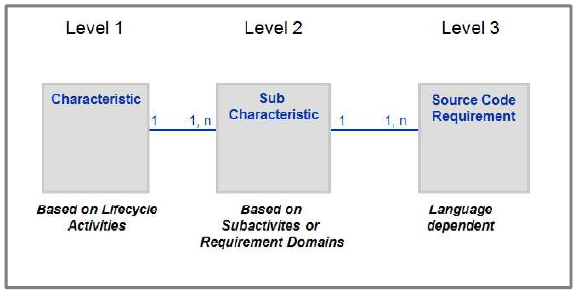
\includegraphics[scale=0.7, trim = 0cm 0cm 0cm 0cm, clip=true]{figSonarCloud/SQALE.PNG}
	\caption{Struttura generale del modello di qualità SQALE}
	\label{fig:sqale}
\end{figure}

\subsection{Caratteristiche}
Il modello di qualità SQALE ha nove caratteristiche di livello 1, come mostrato in \autoref{fig:caratteristiche}. Queste sono “abilità” ricavate dallo standard ISO 25010. Sono state selezionate in primo luogo perché dipendono dalle proprietà interne del codice, ed in secondo luogo perché impattano direttamente le attività tipiche del ciclo di vita dell’applicazione software.

\begin{figure}[htbp]
	\centering
	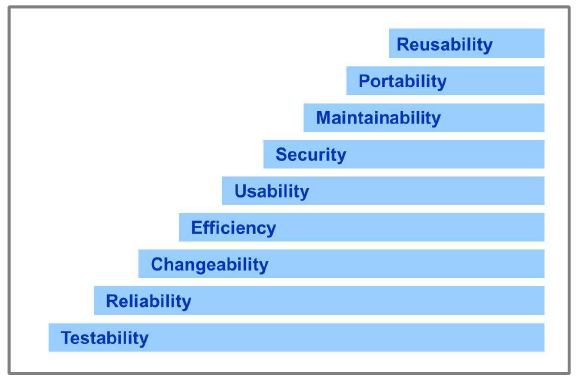
\includegraphics[scale=0.7, trim = 0cm 0cm 0cm 0cm, clip=true]{figSonarCloud/caratteristiche.PNG}
	\caption{Caratteristiche del modello di qualità SQALE}
	\label{fig:caratteristiche}
\end{figure}

Pertanto, il modello di qualità SQALE può essere considerato come una proiezione del modello ISO 25010
nella cronologia del ciclo di vita dell’applicazione software.
\subsection{Sottocaratteristiche}
Ogni caratteristica può essere suddivisa in sotto-caratteristiche le quali sono utilizzate per
combinare i requisiti in gruppi di medie dimensioni in modo tale da eseguire analisi approfondite. Ci sono
due tipi di caratteristiche:
\begin{itemize}
	\item  Sotto-caratteristiche corrispondenti alle attività del ciclo di vita come i test di unità, test
	d’integrazione, ottimizzazione dell’uso dei processori e ottimizzazione della dimensione del codice
	generato. Questi sono rappresentati in \autoref{fig:sub} seguendo il loro ordine cronologico.
	\item Sotto-categorie risultanti dalla generica tassonomia individuata in termini di buone e cattive pratiche
	relative all’architettura e codifica del software. Questa classificazione è una scelta implementativa.
	L’ispirazione può essere guidata da classificazioni esistenti come quella effettuata da D. Spinellis.
\end{itemize}
\begin{figure}[htbp]
	\centering
	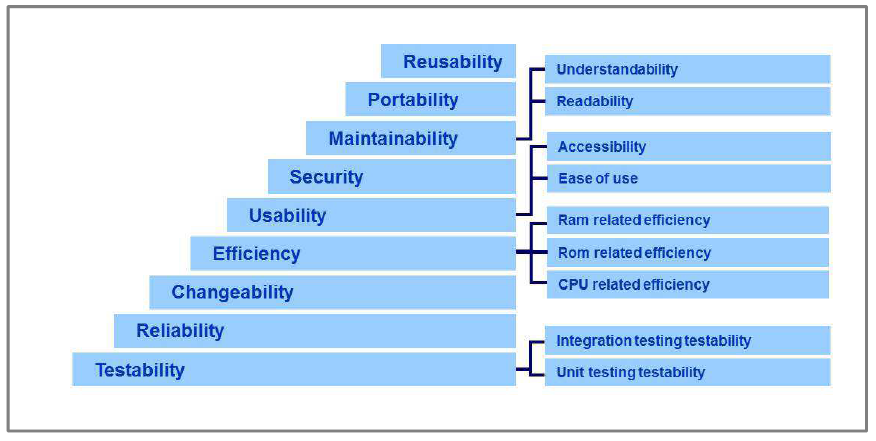
\includegraphics[scale=0.7, trim = 0cm 0cm 0cm 0cm, clip=true]{figSonarCloud/sub1.PNG}
	\caption{Sotto-caratteristiche relative al ciclo di vita}
	\label{fig:sub}
\end{figure}
\subsection{Il livello dei requisiti}
Il livello dei requisiti contiene tutti i requisiti relativi alla qualità del codice. Sono formulati rispettando i
criteri di qualità (atomicità, chiarezza, e così via) definiti in precedenze.
I requisiti sono collegati agli artefatti che compongono il codice sorgente del software in considerazione.
Ognuno di essi sarà collegato con il livello più basso possibile. Ad esempio, si supponga che si stia
esprimendo un requisito relativo alla complessità ciclomatica. Questa proprietà interna impatta sugli sforzi
dei test di unità (quindi la testabilità) e la comprensione (quindi la manutenibilità). Si allegheranno i requisiti
alla prima sotto caratteristica, che è il test di unità e quindi alla testabilità. Un requisito tipico, potrebbe
essere quello di rimanere entro un certo limite di soglia per una misura strutturale, o il rispetto di una regola
sintattica
\section{Il metodo SQALE per la misura del Techical Debt}
A partire dalla sua pubblicazione, risalente al 2010, SQALE è diventato il metodo standard a livello industriale per la gestione del Technical Debt. Gli obiettivi principali di tale metodo sono sostanzialmente i seguenti:
\begin{enumerate}
	\item fornire una stima del costo del technical debt di un pezzo di codice sorgente;
	\item fornire indicatori che consentano un'analisi  dettagliata della natura del debito tecnico;
	\item supportare strategie di rimedio utilizzando indicatori. Esistono molte strategie potenziali e la scelta è dettata dal contesto;
	\item essere implementabili all'interno di una soluzione automatizzata per fornire supporto decisionale in tempo reale.
\end{enumerate}
Al fine di raggiungere tali obiettivi, il metodo SQALE utilizza quattro concetti:
\begin{enumerate}
	\item un modello di qualità;
	\item modelli di stima;
	\item indici;
	\item indicatori.
\end{enumerate}
\subsection{Il modello di qualità}
Il modello di qualità è una lista dei buoni principi che un team o un'organizzazione deve considerare per la definizione di un codice di qualità. Tale lista serve come riferimento per stimare il technical debt del codice. Qualsiasi non conformità con il modello di qualità crea debito e non vi è alcun debito senza la violazione di almeno uno dei requisiti. Se un'organizzazione non vuole definire una lista di questo tipo, oppure non ha a disposizione tempo sufficiente, può utilizzare un modello noto come A2DAM (Agile Alliance Debt Analysis Model) oppure l'elenco predefinito fornito dagli strumenti di analisi statica.
\subsection{Modello di stima}
Il metodo SQALE contiene due modelli di stima. Il primo viene utilizzato per stimare il tempo necessario a rimediare ad ogni debito associato ad ogni item all'interno del codice. Si parla di \textit{remediation cost}. Il secondo modello stima l'impatto del debt sul business e si parla di \textit{non-remediation cost}. Esso stima i costi addizionali futuri e  potrebbe anche essere considerato come il costo legato al rimandare la risoluzione di un problema.
Pertanto, con SQALE, ogni voce di debito ha due costi:
\begin{itemize}
	\item il costo di riparazione,
	\item il costo di non riparazione.
\end{itemize}
Tutti questi calcoli sono eseguiti dagli strumenti di analisi che supportano il metodo.
La maggior parte di questi strumenti ha tali modelli di stima già preconfigurati, quindi è possibile iniziare ad analizzare il codice con le impostazioni predefinite.
Quando si aggiungono tutti i costi di riparazione di tutti gli elementi di debito rilevati dall'analisi del codice, si ottiene il debito tecnico del componente, dell'applicazione o del dominio software. Quando si aggiungono tutti i costi di non rimedio di un componente software, si ottiene l'impatto sul business (la parte di interesse) del componente.
\subsection{Indici}
Gli indici considerati sono due e derivano dai due modelli di stima. In particolare, si considerano:
\begin{itemize}
	\item technical debt index,
	\item business impact index.
\end{itemize}
Questi due indicatori dovrebbero essere monitorati e resi trasparenti a tutti i partecipanti a un progetto in modo tale che ognuno in ogni momento saprà quanto debito tecnico il progetto sta maturando in termini di capitale o interesse. \\ Un altro indice importante è il debt ratio che è il debito tecnico diviso per il budget del progetto. Per tornare alla metafora finanziaria, un modo per valutare lo stato di salute di un'azienda è calcolare il suo rapporto di indebitamento, che è il rapporto tra i debiti e le attività della società. Per analogia, il rapporto di indebitamento SQALE consente di monitorare lo stato di salute dei progetti e delle applicazioni.
\subsection{Indicatori}
L'indicatore maggiormente utilizzato è lo SQALE rating. Sostanzialmente si associa una lettera a determinate percentuali di debt ratio. In particolare, le lettere vanno da A ad E e ad ogni lettera è associato un colore. Si mostra un esempio in \autoref{fig:rating}. Un debt ratio basso produce come risultato A, mentre il grado più alto è E.
\begin{figure}[htbp]
	\centering
	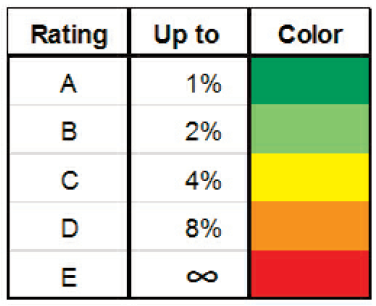
\includegraphics[scale=0.5, trim = 0cm 0cm 0cm 0cm, clip=true]{figSonarCloud/SQUALE1.png}
	\caption{Esempio di griglia del SQALE RATING}
	\label{fig:rating}
\end{figure}
Il secondo indicatore più utilizzato è la piramide SQALE, che rappresenta la distribuzione del debito tecnico in termini di caratteristiche di qualità come mostrato in \author{fig:piramide}. Questo indicatore può essere letto in due modi:
\begin{enumerate}
	\item  La vista analitica (rappresentata dai numeri nella colonna di sinistra e dalle barre di colore azzurro)
	\item La vista consolidata (rappresentata dai numeri nella colonna destra e dalle barre blu scuro)
\end{enumerate}

\begin{figure}[htbp]
	\centering
	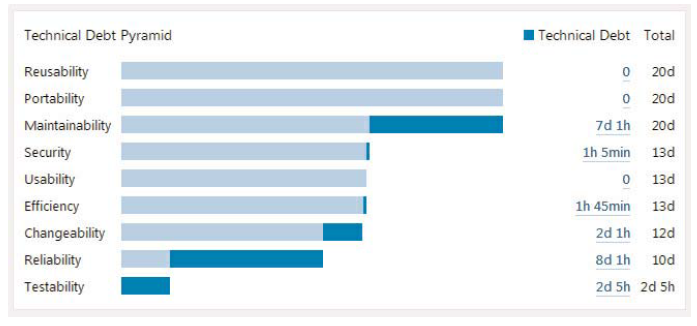
\includegraphics[scale=0.5, trim = 0cm 0cm 0cm 0cm, clip=true]{figSonarCloud/piramide.PNG}
	\caption{La piramide SQALE}
	\label{fig:piramide}
\end{figure}
La vista consolidata della piramide, si ottiene sommando il debito di tutti i livelli caratteristici inferiori per una data caratteristica.
Questi calcoli sono indicati dai numeri nelle colonne di destra. Si prenda ad esempio l'utilità,che ha un debito tecnico di 12 giorni. I progetti agili generano un numero elevato di cicli di modifica del codice. Le caratteristiche qualitative necessarie per supportare questi sviluppi sono la testabilità, l'affidabilità e la variabilità.
Poiché la variabilità si basa sull'affidabilità e sulla testabilità, la distanza reale tra lo stato corrente del codice e lo stato di destinazione del codice facilmente modificabile è la somma del debito associato a ciascuna delle tre caratteristiche (2d 5h + 8d 1h + 2d 1h = 12d). Questo valore consolidato risponde alla seguente domanda di un rappresentante aziendale: "Quanto siamo lontani dall'avere software modificabile?" Questo meccanismo di consolidamento è applicabile a tutte le caratteristiche
Altro indicatore SQALE è la mappa del debito SQALE. Si tratta di un grafico a bolle su cui un l'item (un file, un componente, un'applicazione) è rappresentato su due assi, il debito tecnico e l'impatto sul business, come mostrato in \autoref{fig:bolle}. 
\begin{figure}[htbp]
	\centering
	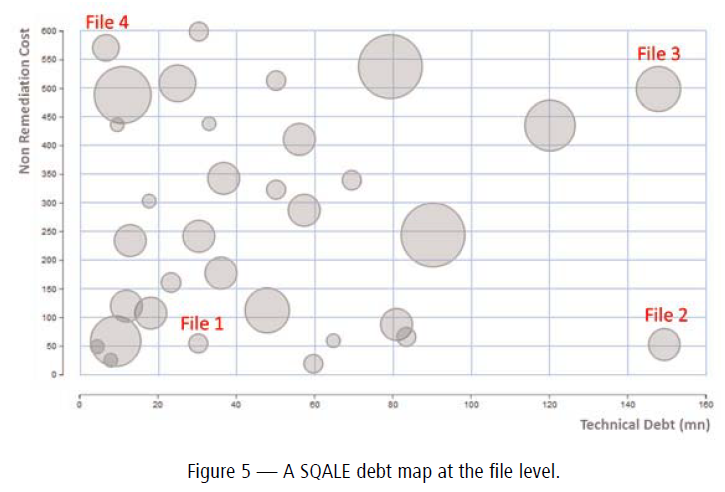
\includegraphics[scale=0.5, trim = 0cm 0cm 0cm 0cm, clip=true]{figSonarCloud/bolle.PNG}
	\caption{La piramide SQALE}
	\label{fig:bolle}
\end{figure}
%Tale metodo è basato esclusivamente su regole e questo significa che se si vuole gestire tutto il technical debt con SQALE, bisogna prima abilitare le regole nel repository Common SonarQube che contrassegna:
%\begin{itemize}
%\item blocchi duplicati;
%\item casi di test falliti;
%\item numero di casi di test insufficiente a coprire i branch;
%\item densità di commenti insufficiente;
%\item numero di test insufficiente a coprire le linee di codice;
%\item casi di test saltati.
%\end{itemize}
%Tali regole si trovano nel repository Common SonarQube perché sono comuni a tutte i linguaggi di programmazione. Una volta abilitate è possibile tenere traccia di tutti i difetti di qualità e monitorare il debito tecnico, che il metodo SQALE misura in giorni.

%\subsection{Il metodo Sqale}
%Il metodo SQALE è stato sviluppato per rispondere a un'esigenza generica e permanente di valutazione della qualità del codice sorgente visto che standard come ISO 9126 e ISO / IEC 15939 non forniscono un supporto efficace. Si tratta di un metodo generico ed indipendente da linguaggio e strumenti. Esso permette di:
%\begin{itemize}
%\item definire chiaramente cosa crea il debito tecnico;
%\item stimare correttamente il debito;
%\item analizzare tale debito dal punto di vista tecnico e di business;
%\item offrire strategie di prioritizzazione diverse che consentono di stabilire un piano di ammortamento ottimale. 
%\end{itemize}
%Il modello di qualità SQALE viene utilizzato per formulare e organizzare i requisiti non funzionali relativi alla qualità del codice. È organizzato in tre livelli gerarchici:
%\begin{enumerate}
%\item il primo livello è composto da caratteristiche;
%\item il secondo di sotto-caratteristiche;
%\item il terzo livello è composto da requisiti relativi agli attributi interni del codice sorgente.
%\end{enumerate}
%Tali requisiti di solito dipendono dal contesto e dalla lingua del software. Qualsiasi violazione di questi requisiti induce il debito tecnico.